\documentclass[conference]{IEEEtran}
\usepackage[spanish]{babel}
\usepackage[utf8]{inputenc}
\usepackage{blindtext, graphicx}
\usepackage{subfigure}
\usepackage{mdwmath}
\usepackage{mdwtab}
\usepackage{subfig}
\usepackage{amsmath}
\usepackage{array}
\usepackage{multirow}
\bibliography{myBibliography}

\begin{document}
\title{  Clasificación De Canciones Por Género Utilizando Una Red Neuroral Artificial Y La API De Spotify }
\author{\IEEEauthorblockN{Moreno Vázquez Pedro Abraham}
\IEEEauthorblockA{Departamento de Estudios Multidisciplinarios\\ Divisi\'on de ingenier\'ias\\
Campus Irapuato-Salamanca\\
Yuriria, Guanajuato\\
Correo: pa.morenovazquez@ugto.mx}

\and
\IEEEauthorblockN{Moreno Ramírez Walter Alejandro }
\IEEEauthorblockA{Departamento de Estudios Multidisciplinarios\\ Divisi\'on de ingenier\'ias\\
Campus Irapuato-Salamanca\\
Yuriria, Guanajuato\\
Correo: wa.morenoramirez@ugto.mx}}

\maketitle
\renewcommand\abstractname{Abstract}
\begin{abstract}
Here we go. \\
\end{abstract}

\begin{IEEEkeywords}
Keywords
\end{IEEEkeywords}

\IEEEpeerreviewmaketitle
\section{Introducción}
En la búsqueda de entender y replicar los sentidos que tenemos los seres humanos; su funcionamiento, procesamiento de la señal y el entendimiento de como nuestro cuerpo humano percibe e interpreta el mundo exterior, la ciencia se ha encargado de replicar y, en algunos casos, mejorar los sentidos que poseemos o de recuperar sentidos como el oido o el tacto en miembros humanos inutilisables o perdidos. Pero todo va aún más allá, existen ciencias encargadas de estudiar como se genera el conocimiento, la conciencia y como es el proceso dentro de nuestro cerebro cuando se esta realizando una acción tan cotidiana como es el escribir, hablar o un proceso aún más complejo como lo es el aprender. "Todos los procesos del cuerpo humano se relacionan en alguna u otra forma con actividad de neuronas. Las neuronas son un componente relativamente simple del ser humano, pero cuando millones de ellas se conectan en forma conjunta se hacen muy poderosas. \\
Lo que básicamente ocurre en una neurona biológica es lo siguiente: la neurona es estimulada o excitada a través de sus entradas (inputs) y cuando se alcanza un cierto umbral, la neurona se dispara o activa, pasando una señal hacia el axon. Así, el secreto de la "inteligencia", se sitúa dentro de estas neuronas interconectadas y de su interacción.\\

Por lo tanto, las Redes Neuronales biológicas:

\begin{itemize}
	\item Consisten en unidades de procesamiento que intercambian datos o información.
	\item Se utilizan para reconocer patrones, incluyendo imágenes, manuscritos y secuencias de tiempo.
	\item Tienen capacidad de aprender y mejorar su funcionamiento."[1]
\end{itemize}

\subsection{Redes Neuronales Artificiales \\}


\subsection{API Web de Spotify \\}
La API web de Spotify permite a los desarrolladores utilizar su aplicación para obtener datos del catálogo de música de Spotify. Los resultados de las peticiones a los servidores de Spotify dan como resultado archivos en formato JSON que proporciona información como artistas, álbumes y pistas directamente desde el catálogo de Spotify. Dependiendo de la autorización del usuario, la API también puede proporcionar a los programadores acceso a datos relacionados con el usuario, es decir, listas de reproducción y músicas guardadas en la biblioteca del usuario.\\

\begin{figure}[ht]
    \centering
    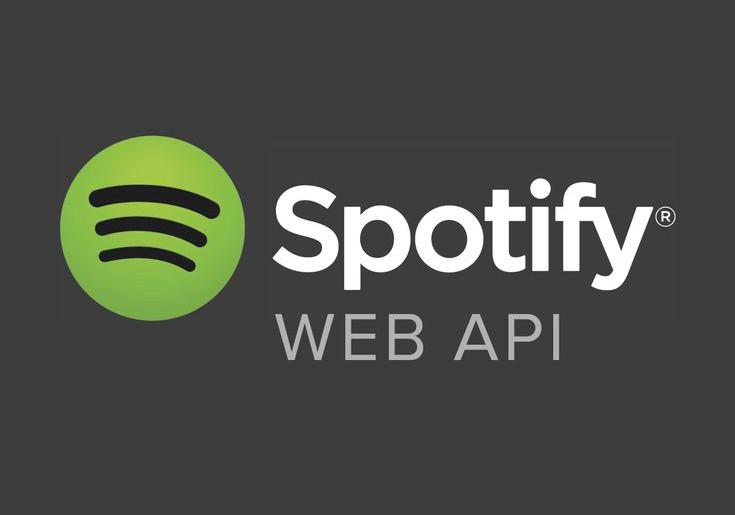
\includegraphics[width=1.8in]{./images/APIWebSpotify.jpg}
    \DeclareGraphicsExtensions.
    \caption{ Logo oficial de la API Web de Spotify. }
\end{figure}

Con la API web de Spositfy se pueden crear aplicaciones basando la lógica de negocio en el catálogo de música de Spotify. Estas aplicaciones son básicamente aplicaciones web integradas en el navegador basado en Chromium y bajo el sandbox que incluye Spotify. El desarrollo de una aplicación de Spotify es prácticamente idéntico que cualquier aplicación HTML5 que se crea hoy en día. Se puede combinar todo el conjunto de herramientas que se tienen a disposición como CSS, HTML y Javascript, así como cualquier framework Javascript como jQuery.

\subsection{Objetivo principal}
La finalidad de este trabajo es, mediante la utilización de una Red Neuronal Artificial (ANN), clasificar un conjunto de canciones en uno de cuatro géneros posibles: Metal, Mexicano, Pop y Rock. Utilizando la ANN para realizar las etapas de entrenamiento y pruebas. Comparando los resultados de la ANN con el algoritmo del vecino más cercano.\\

\section{Metodolog\'ia}
La conexión a los servidores de Spotify a través de su API, se realiza con scripts de Node.js, donde se realiza una autorización por parte del usuario para acceder a los datos. Para comenzar a realizar las peticiones se deben especificar dos claves que se generan para cada cuenta de desarrollador. Con estas claves un desarrollador se puede autenticar ante Spotify como usuario de su servicio, estas claves son: Client ID y Client Secret.\\

La API de Spotify permite, además de generar una estadística muy completa del uso de las canciones, obtener las características musicales de cada canción, ya sea de manera individual o en conjunto, mediante una playlist.\\
La características que se pueden obtener utilizando la API de Spotify son los siguientes: \\

\begin{itemize}
	\item Danceability
	\item Energy
	\item Key
	\item Loudness
	\item Mode
	\item Speechiness
	\item Acousticness
	\item Instrumentalness
	\item Liveness
	\item Valance
	\item Tempo \\
\end{itemize}

Se crearon 4 Playlist en Spotify, las cuales hacen referencia a cada género musical que se desea clasificar. A cada Playlist se agregó un total de 40 canciones, teniendo en total 160 canciones de muestras, de las cuales se obtuvieron sus características musicales como se mencionó anteriormente. Del total de canciones 120 (30 de cada Playlist) se tomarán para la etapa de entrenamiento y 40 (10 de cada Playlist) para la etapa de pruebas.\\

\begin{figure}[htbp]
	\centering
	\subfigure{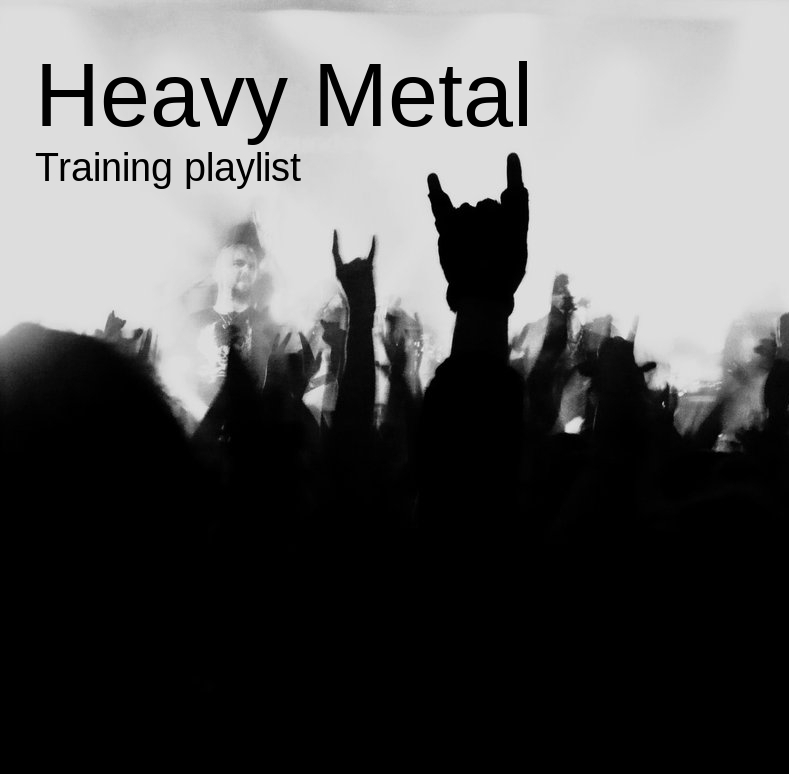
\includegraphics[scale=0.15]{./images/heavyMetalPlaylist.jpg}}
	\subfigure{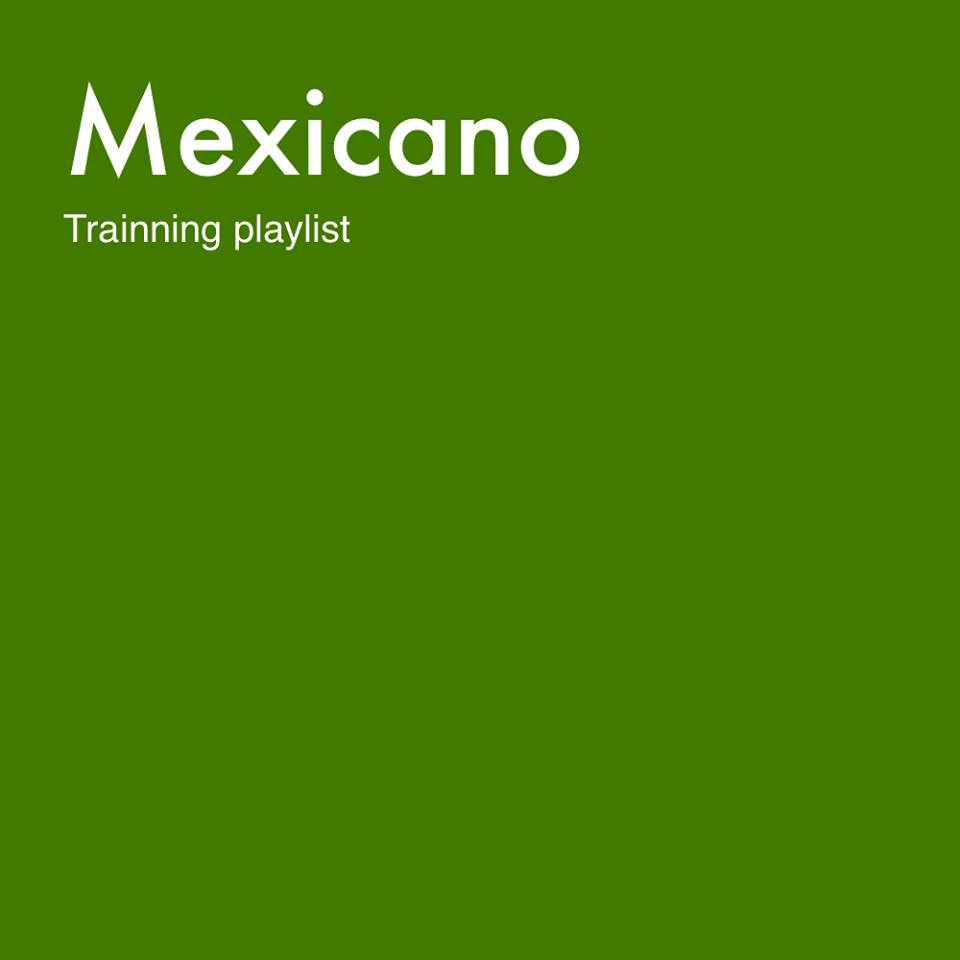
\includegraphics[scale=0.121]{./images/mexicanoPlaylist.jpg}}
	\subfigure{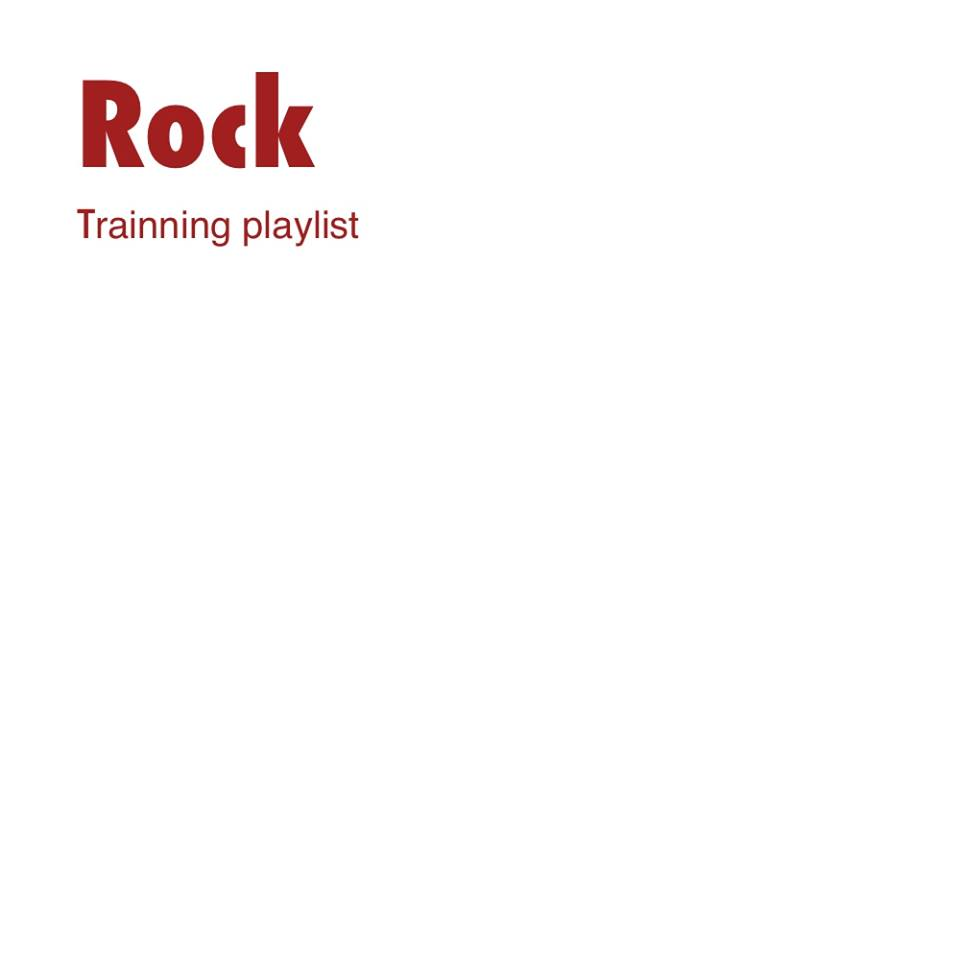
\includegraphics[scale=0.125]{./images/rockPlaylist.jpg}}
	\subfigure{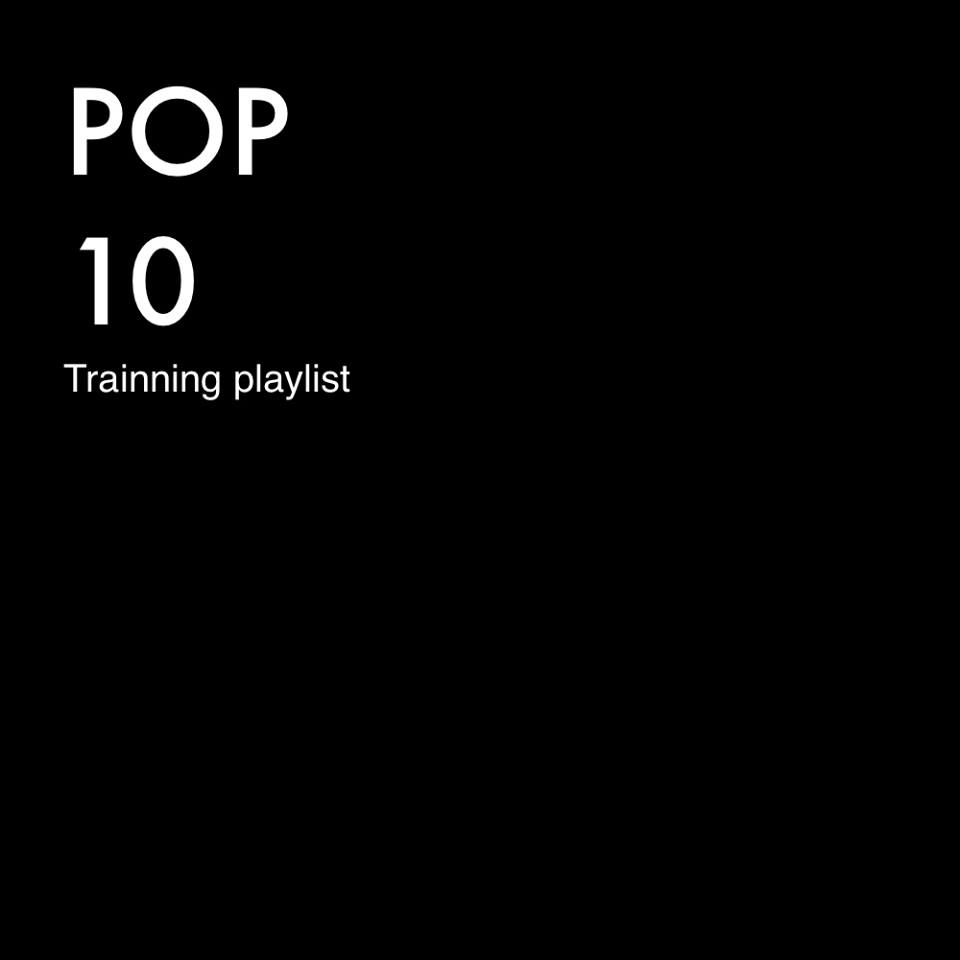
\includegraphics[scale=0.125]{./images/popPlaylist.jpg}}
	\caption{ Caratulas de las playlist creadas para ordenar las canciones que se utilizarán para entrenamiento y pruebas. }
\end{figure}

Spotify genera un ID único para cada usuario, canción, playlist, etc., el cual sirve para hacer referencia a cada elemento dentro de los servidores de Spotify. Proporcionando las claves Client ID, Client Secret, el id de la playlist y la canción, se pueden solicitar todas las características anteriormente mencionadas de cada canción de las 4 playlist. Para realizar este procedimiento, se creó un script de Node.js, con el cual se obtienen las once características para cada canción de las 4 playlist.\\

\subsection{Etapa de entrenamiento}
Una ves obtenidas las características de cada canción, se adecuan al formato ARFF (Attribute-Relation File Format) de Weka, siendo este el archivo con el que se alimenta la Red Neuronal Artificial para la etapa de entrenamiento.\\
Dentro de la configuración de Weka, se selecciona, como método de clasificación, una Red Neuronal de un Perceptron Multicapa para realizar la etapa de entrenamiento.\\

Weka da la oportunidad de realizar una validación cruzada. Para esta opción, se selecciona el 25 \% del total de canciones, correpondiendo a 120 canciones que se utilizarán para esta etapa de entrenamiento.



\subsection{Etapa de pruebas}
La etapa de pruebas se debe realizar con elementos que no pertenezcan a los conjuntos de datos etiquetados que se utilizaron en la etapa de entrenamiento, esto para que el resultado sea justamente una prueba del algoritmo y la implementaci\'on ya que, de utilizarse un elemento perteneciente al conjunto de datos etiquetados para una clase en espec\'ifico arrojar\'ia un resultado esperado.\\

Para comparar la exactitud de la red neuronal, se implementó el algoritmo del vecino m\'as cercano, utilizado en la etapa de pruebas de los métodos de clasificación supervizada. Este m\'etodo consiste en obtener la distancia euclidiana, Ecuaci\'on (1), entre el elemento de prueba con cada una de las cuatro clases.

\begin{equation}
	D = \sqrt{ (C_n - S_{1} )^2 + (C_n - S_{2} )^2 + ... + (C_n - S_{11} )^2 }
\end{equation}

Donde:\\
\begin{itemize}
	\item $d$: es la distancia entre la canción de entrada y el prototipo de una de las 4 clases.
	\item $C_n$: es el prototipo para cada clase.
	\item $n = 1, 2, 3, 4$: indica el número de cada clase.
	\item $S_{1}, S_{2}, S_{3} ... S_{11}$: son las características de la canción de entrada. \\
\end{itemize}

La clasificación de cada nueva canción, utilizando este algoritmo, se hará con la distancia menor de las tres distancias calculadas ya que es a la clase que más se acerca de acuerdo a sus características obtenidas con la API de Spotify.\\\\

\section{Resultados}

Detallar bien los datos obtenidos de la Red Neuronal \\

**** Agregar la matriz de confusion y explicarla a detalle \\\\

\begin{table}[h]
\renewcommand{\arraystretch}{1.3}
\renewcommand{\tablename}{Tabla}
\caption{ Porcentaje de canciones clasificadas utilizando el algoritmo del vecino más cercano. }
\label{table_example}
\centering
\begin{tabular}{|c|c|c|}
\hline
CLASE (género) & Correctas & Incorrectas \\
\hline
Clase 1 (Metal) & 50.0 \% & 50.0 \% \\
\hline
Clase 2 (Mexicano) & 0.0 \% & 100.0 \% \\
\hline
Clase 3 (Pop) & 0.0 \% & 100.0 \% \\
\hline
Clase 4 (Rock) & 40.0 \% & 60.0 \% \\
\hline
Total & 22.50 \% & 77.50 \% \\
\hline
\end{tabular}
\end{table}

La Tabla I. muestra el resultado del algoritmo del vecino más cercano. La información que nos proporciona este tabla, indica el grado de exactitud con el que el algoritmo del vecino más cercano puede clasificar una nueva canción. \\

\section{Concluciones}

\begin{thebibliography}{1}
\item [[1]] % Matich, D. J. (2001). Redes Neuronales: Conceptos Básicos y Aplicaciones. Historia, 55. Retrieved from https://www.frro.utn.edu.ar/repositorio/catedras/quimica/5_anio/%orientadora1/monograias/matich-redesneuronales.pdf
\end{thebibliography}



\end{document}